\chapter{Présentation du projet}

	\section{Présentation de l'application}

    Puzzle Edition est une application de jeu, dotée d'une interface graphique, qui consiste à assembler des formes de sorte qu'elles occupent le moins de place possible. Cela s'apparente au tetrix, mais avec des modalités différentes. D'ailleurs, le joueur retrouvera certaines pièces de ce jeux. Ces pièces peuvent être placer, déplacer ou supprimer du plateau ou encore tourner.

    Le joueur peut créer ou charger une partie. La difficulté de la partie est mesurer en fonction de la taille du plateau choisis ainsi que le nombre de pièces générés. En effet, plus il y a de pièces généré, plus la partie est difficile, mais plus le score sera élevé. C'est pour cela qu'à chaque partie, il est possible soit de demander à obtenir une nouvelle configuration de départ, soit charger une configuration déjà créée et sauvegardée.

    Le but du joueur est de minimiser l'espace occupé par l'ensemble des pièces. Plus précisément, la fonction d'évaluation sera l'aire du plus petit rectangle (parallèle aux axes) recouvrant l'ensemble des pièces. Lorsque le joueur considère avoir terminé (ou lorsque le nombre maximum d'actions autorisées est atteint), il clique sur un bouton est son score est alors calculé.

    Une option permet de faire jouer l'ordinateur sur une nouvelle partie, ou une partie déjà sauvegarder, permettant ainsi de comparer son score avec celui de l'ordinateur.

    \begin{table}[h]
        \centering
        \begin{tabular}{cc}
            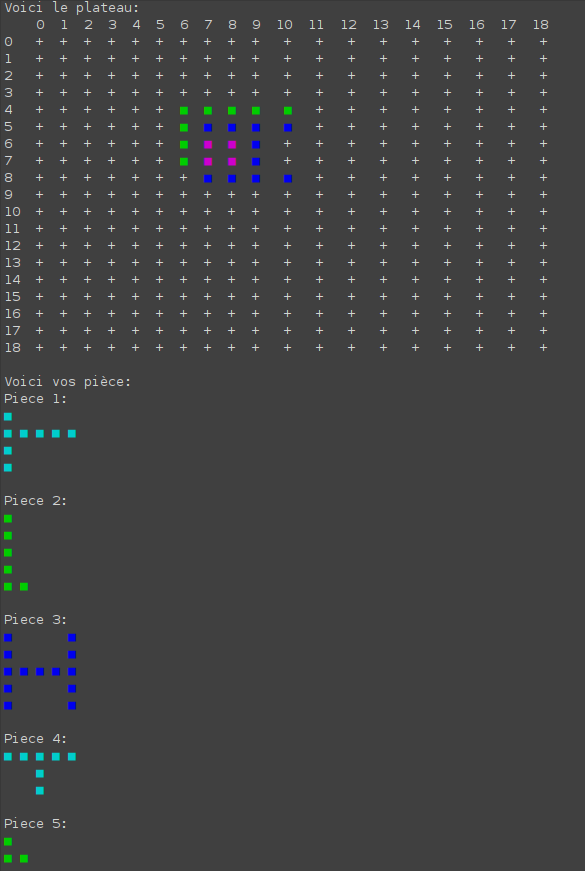
\includegraphics[width=0.40\textwidth, keepaspectratio]{img/vueConsole.png} & 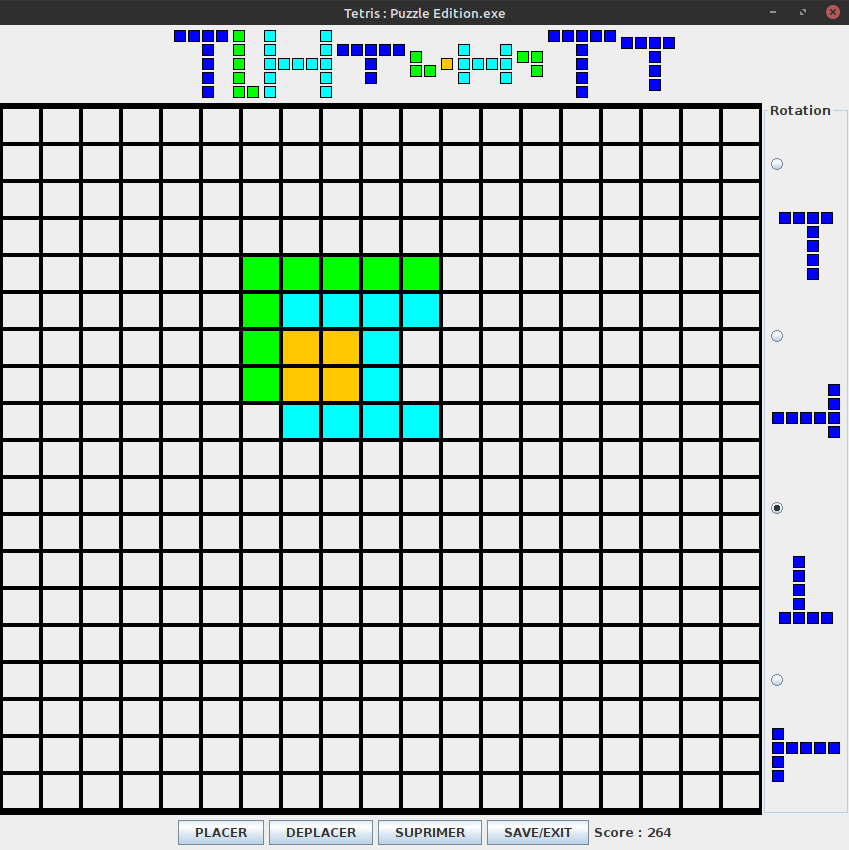
\includegraphics[width=0.40\textwidth, keepaspectratio]{img/vueGraphique.png}\\
            Vue console & Vue graphique\\
        \end{tabular}
   \end{table}
